\documentclass{article} % For LaTeX2e
\usepackage{nips15submit_e,times}
\usepackage[colorlinks,linkcolor=red]{hyperref}
\usepackage{url}
\usepackage{amsmath}
\usepackage{graphicx}
\usepackage{float}
\usepackage{bm}
\usepackage{amssymb}
%\documentstyle[nips14submit_09,times,art10]{article} % For LaTeX 2.09


\title{CS499 Homework 11 (First Draft)}


\author{
	Intersteller\thanks{ Use footnote for providing further information
		about author (webpage, alternative address)---\emph{not} for acknowledging
		funding agencies.}
	Department of Computer Science
	Cranberry-Lemon University
	Pittsburgh, PA 15213
}

% The \author macro works with any number of authors. There are two commands
% used to separate the names and addresses of multiple authors: \And and \AND.
%
% Using \And between authors leaves it to \LaTeX{} to determine where to break
% the lines. Using \AND forces a linebreak at that point. So, if \LaTeX{}
% puts 3 of 4 authors names on the first line, and the last on the second
% line, try using \AND instead of \And before the third author name.

\newcommand{\fix}{\marginpar{FIX}}
\newcommand{\new}{\marginpar{NEW}}

\newtheorem{theorem}{}

%\nipsfinalcopy % Uncomment for camera-ready version

\begin{document}
	
	
	\maketitle
\textbf{Exercise 11.1}\par

	 As we have proved in \textbf{Exercise 8.8}, the largest antichain of $\{0,1\}^n$ is $\binom{n}{\lfloor n/2\rfloor}$. \par

	 We define a layer as a set of strings containing same number of $'1'$ and is sorted by how many  $'1'$ a string in this layer contains.\par

	 \textbf{1.}There are $\binom{n}{\lfloor n/2\rfloor}$ strings in the middle layer, which has the most strings. Since any two strings from the same layer are not comparable, there are at least $\binom{n}{\lfloor n/2\rfloor}$ chain partitions.\par

	 \textbf{2.} All strings in any layer except the middle one can form chains with unique strings in its adjacent layer with the following method:\par

	 Since $0\le k < n/2 $, there are more $'0'$ than $'1'$ in this layer, we calculate a strings score by the following rules: scan the string from the beginning and the initial score is $0$, add one if current digit is $0$,minus one otherwise. Find the digit where the first highest score appears (which must be a $'0'$),change it to $1$. Then we get a string belongs to its adjacent layer and these two strings can form a chain(they are comparable).Now we prove that this string is unique:\par

	 Assume that there are two different strings that transform into a same string. Assume that the first string changes the i-th digit, and the other changes the j-th digit (with no loss of generality, assume $i<j$).  Then the i-th digit of the second string and the j-th digit of the first string are $0$, whereas other digits are the same. Assume that the score of the $(i-1)$-th digit is k.Then the score of the i-th digit is $k+1$ for the first string and $(k-1)$ for the second. Assume that the score of the $(j-1)$-th digit for the first string is $k+1+p$,then the score of the $(j-1)$-th digit for the second string is $k-1+p$.The score of the j-th digit for the second string is $k+p$. Since the changing digit is where the first largest score occurs, we have

	 $$
	 k+1 \ge k+1+p
	 $$

	 $$
	 k<k+p
	 $$

	 where we get $p\leq 0$ and $p>0$ which contradict each other. So  different strings cannot transform into a same string by the method.\par
	
	 Accordingly, we can get a matching of size $(^n _k)$ between the k-th layer and the $(k+1)$-th layer.
\textbf{Exercise 11.2}\par
	This case, $|\Gamma(A)|\ge |A|$ for every $A\subseteq L$. We use contradiction to prove it.
	Assume $|\Gamma(A)|<|A|$, $\exists A\subseteq L$. Since every vertex has degree $d$, consider $A$, we have $d\times |A|$ edges.
	Since $\frac{d\times|A|}{|\Gamma(A)|}>d$, there must exist a vertex in $R$ which degree is larger than $d$. It is a contradiction.
	Therefore, $|\Gamma(A)|\ge |A|$ for every $A\subseteq L$. According to course video, if $|\Gamma(A)|\ge |A|$ for every $A\subseteq L$,
	then (and only then) there exists a matching of size $|L|$. $G$ has a perfect matching.\par 	


\textbf{Exercise 11.3}\par
    Based on the mathematical induction, we have:\par
    $(1)$ When $d=1$, obviously the edges $E(G)$ can be partitioned into $d$ perfect matchings.\par
    $(2)$ When $d>1$, we suppose when $d=n$, the edges $E(G)$ can be partitioned into $d$ perfect matchings. When $d=n+1$, we can find a matching $M$ of size $|L|$ based on the $11.2$, now we delete $M$ from $E(G)$ and we get a new bipartite graph $G\prime$ whose every vertex has degree $n$. Based on the inductive assumption, the edge $E(G\prime)$ can be partitioned into n perfect matchings. We can add $M$ to $M_1,\cdots,M_n$ and get matchings $M_1,\cdots,M_{n+1} \subset E(G)$ such that $(1) M_i \cap M_j = \emptyset for 1\leq i<j\leq n+1$ and $(2) M_1\cup M_2 \cup\cdots\cup M_{n+1} = E(G)$.\par
    Therefore, if G is a $d$-regular bipartite graph, the edges $E(G)$ can be partitioned into $d$ perfect matchings.

\textbf{Exercise 11.4}\par
    $1.$ For every vertex $X \in V$, add $X\prime$ to constitute $V\prime$. If the capacity of $X$ is $c(X)$ in $G$, the capacity of $edge(X,X\prime)$ in $(G\prime)$ is $c(X).$ If $edge(X,Y)\in E$, $edge(X\prime,Y)\in E\prime$ and $c(X\prime,Y)$ is $\infty$.If the original flow is from s to t, then the flow in $G\prime$ is from s to $t/prime$.\par
    $2.$
    \begin{figure}[H]
  	\centering
  	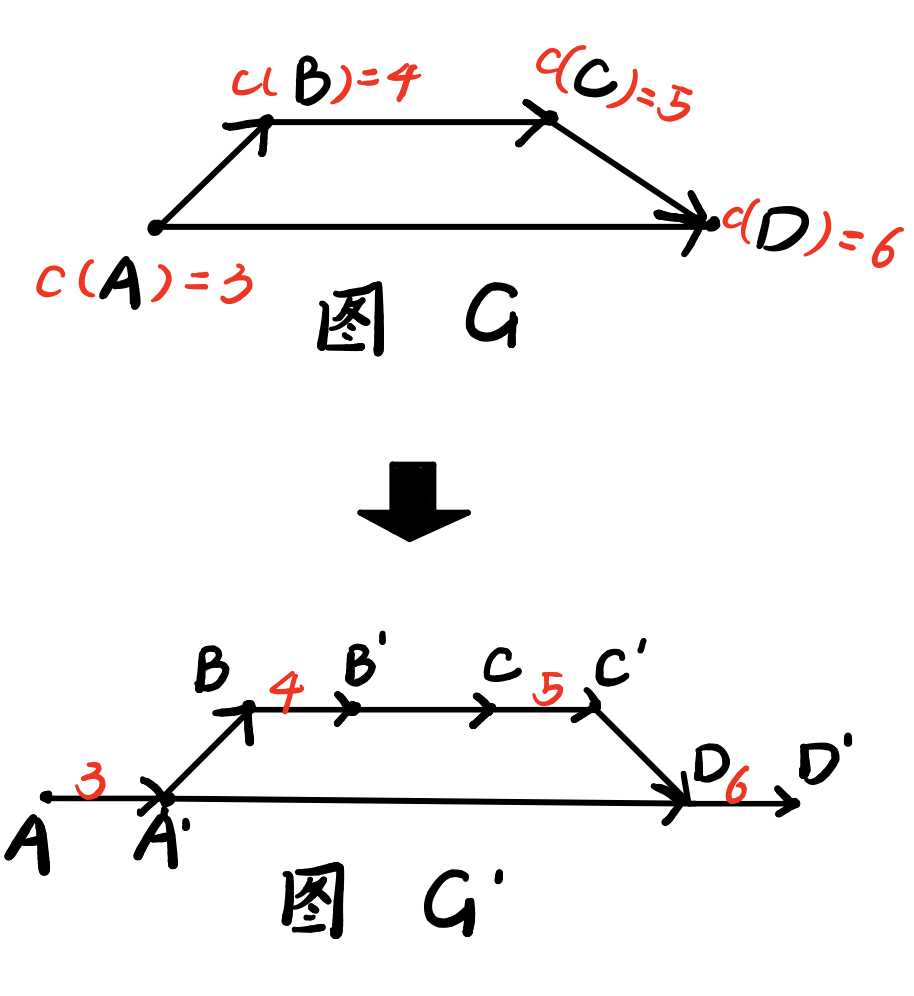
\includegraphics[width=9cm]{11_4_2.png}
  	\caption{}
  	\label{}
  	\end{figure}
    
    
    $3.$ We can set the capacity of every vertex in $G$ as $1$ and transform $G = (V,E,c)$ into a network $G\prime = (V\prime,E\prime,c\prime)$ by the method we give in $11.4.1$. Then we use Edmonds-Karp algorithm on the network. If the maximum flow is k, we find $k$ paths $p_1,p_2,\cdots p_k$, each from $s$ to $t$, such that the paths are internally vertex disjoint.

    \textbf{Exercise 11.5}\par	
	In the i-th layer, there are $(^n _i)$ vertexes, for each vertex, we can form a path that ends at the $(n-i)$-th layer with the method we show in \textbf{Exercise 11.1}. When we reach a layer with more '1' than '0', we can still use this method to form a matching for the following reason. Since we begin at the i-th layer$(i<n/2)$, we have $(n-i)$ '0's and i '1's, so the score of the last digit equals $(n-2i)$, each time we reach the next layer, the max score minus 1 for the  digits before the changing digit remains unchanged. Totally we cross $(n-2I-1)$ layers from the i-th layer to $(n-i)$-th layer, so before we reach the $(n-i)$-th layer, the max score of every string in such path is always positive, which means the algorithm is feasible. Therefore, we can find $(^n _i)$ paths as requested.



\textbf{Exercise 11.6}\par
	1. $e$ is always full. $b$, $c$, $d$, $f$, $g$, $h$, $i$ is sometimes full. $a$ is never full.\par
	2. $e$ is always crossing. $a$, $b$, $c$, $d$, $f$, $g$, $h$, $i$ is never crossing.\par
	
\textbf{Exercise 11.7}\par
	It is impossible to be always full and never crossing.\par
	Proof: Consider an edge $e$ which is always full. We assume the max flow is $MAX$ and $f(e)=c(e)$. We delete this edge and the max flow of residual network is $MAX-c(e)$.
	There must exist minimum cut $MAX-c(e)$ in residual network. We add edge $e$ to this cut and will get minimum cut $MAX$ in original network. Therefore, edge $e$ can be crossing and  is impossible to be a never-crossing edge.\par
	It is impossible to be sometimes full and always crossing, sometimes full and sometimes crossing, never full and always crossing, never full and sometimes crossing.\par
	Proof: These four cases can be proved together. No matter whether it is sometimes full or never full, the edge $e$ can be not full. We assume the max flow is $MAX$ and
	$f(e)=m<c(e)$. If edge $e$ belongs to a minimum cut, delete it and the max flow of residual network is $MAX-m$. The minimum cut $MAX-m$ of the residual network is $MAX-m$. If edge $e$ can be crossing, then the minimum cut in the original network will be $MAX-m+c(e)>MAX$, which controdicts the max-flow-min-cut theorem, so it is not the minimun cut. Therefore edge $e$ is never crossing. \par
	It is possible to be sometimes full and never crossing, never full and never crossing.\par
	Example:\par
    \begin{figure}[H]
  	\centering
  	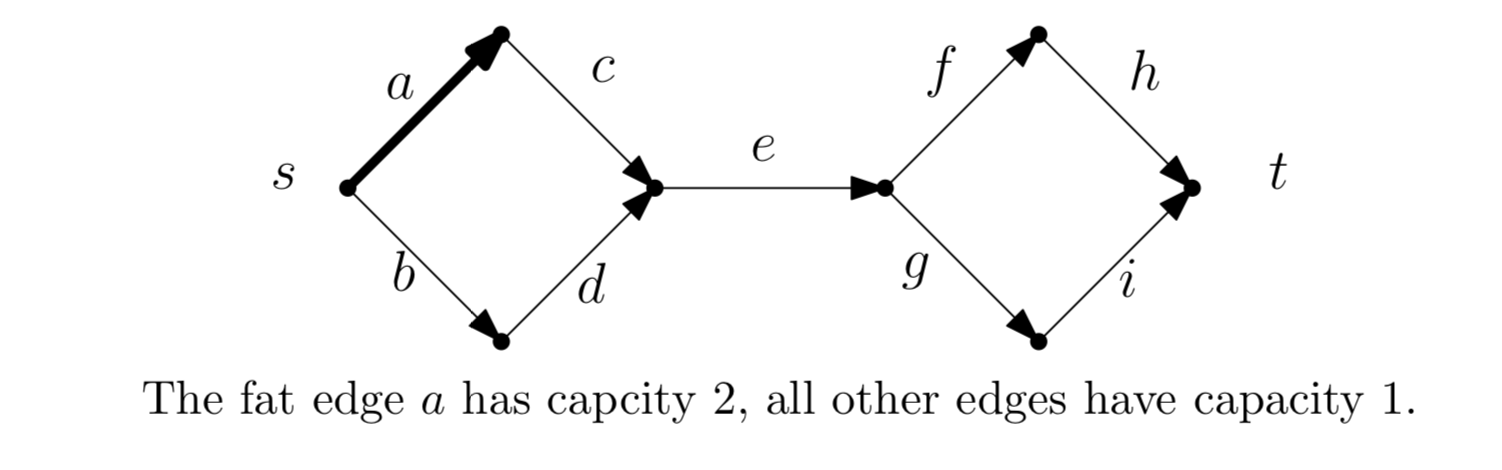
\includegraphics[scale=0.5]{1.png}
  	\caption{}
  	\label{}
  	\end{figure}
	
	In this network, $b$, $c$, $d$, $f$, $g$, $h$, $i$ is sometimes full and $a$ is never full. And $a$, $b$, $c$, $d$, $f$, $g$, $h$, $i$ are all never crossing.\par
	
\end{document}